% =======================================================================
\section{Testing for Failures Refinement -- an Example}
\label{sec:case}
% =======================================================================


For implementing the test case $U_F(p)$ with sub-processes $U_F(p,s)$, it is
advisable to avoid an enumeration of traces $s$ of the reference process.
Instead, we calculate the following auxiliary functions from $P$'s transition
graph.
%
\begin{eqnarray*}
\text{\it initials} & : & N \fun \power (\Sigma)
\\
\minhits & : & N \fun \power\power(\Sigma)
\end{eqnarray*}
%
As mentioned, in a state $n = G(P)/s$, the set $\text{\it initials}(n)$
equals the events labelling outgoing edges of $n$, so  $\text{\it
initials}(n) = [P/s]^0$. The function $\minhits$ maps $n$ to the set of all
minimal hitting sets associated with the minimal acceptances of $n$, so
$\minhits(n) = \minhits(P/s)$. Using the transition function $t$ and the
above functions, $U_F(p)$ can be re-written as the failures-equivalent CSP
process below.
%
\begin{eqnarray}
U_F^1(p) & = & U_F^1(p,0,\ii n)
\\
U_F^1(p,k,n) & = & \big(\Extchoice e:(\Sigma - \text{\it initials}(n)) @ e \then \efail\then \Stop \big)
\label{eq:xufa}
\\ & & \extchoice \nonumber
\\ & & (\minhits(n) = \varnothing) \& \big( \epass \then \Stop \big)
\label{eq:xufb}
\\ & & \extchoice \nonumber
\\ & & (k < p) \& \big(\Extchoice e:\text{\it initials}(n) @ e \then U_F^1(p,(k+1),t(n,e)) \big)
\label{eq:xufc}
\\ & & \extchoice \nonumber
\\ & & (k = p) \& \big( \sqcap_{H\in\minhits(n)} (\Extchoice e:H @ e \then \epass \then\Stop ) \big)
\label{eq:xufd}
\end{eqnarray}
\fixme{alcc: I think the example should be for the theory presented before,
not with a different notion of test. In particular, 33 is very different.}

% .....................................................................................
 \begin{figure}
 %%\hspace*{-40mm}
 \begin{center}
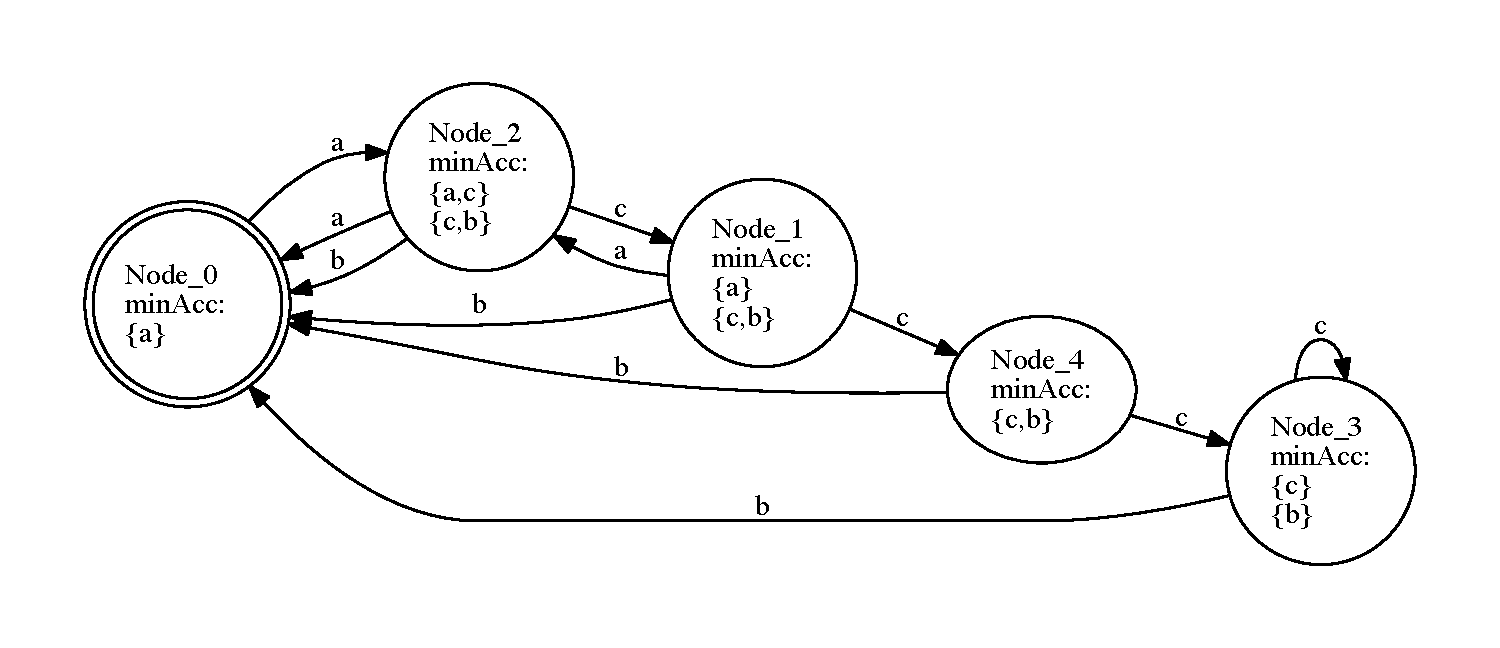
\includegraphics[width=\textwidth]{z_acc.pdf}
\end{center}
%%\vspace*{-10mm}
\caption{Normalised transition graph of faulty implementation $Z$  from Example~\ref{ex:uf1tests}.}
 \label{fig:tgZ}
 \end{figure}
% .......................................................................................

\begin{example}
\label{ex:uf1tests} Consider the following implementation $Z$ of process $P$
from Example~\ref{example:CSP} that is erroneous from the point of view of
failures refinement.
\begin{eqnarray*}
Z & = & a \then (Q_1 \intchoice R_1(r_{max},0))
\\
Q_1 & = & a\then Z \extchoice c\then Z
\\
R_1(r_{max},k) & = & (k < r_{max}) \& \big(b\then Z \extchoice  c\then R_1(r_{max},k+1)\big)
\\ & & \extchoice
\\ & & (k = r_{max}) \& \big(b\then Z \intchoice c\then R_1(r_{max},r_{max})\big)
\end{eqnarray*}
It is easy to see (and can be checked with FDR) that $Z$ is trace-equivalent
to $P$. While $k < r_{max}$, $Z$ also accepts the same sets of events as $P$.
When $R_1(r_{max},k)$ runs through several recursions and $k = r_{max}$ is
fulfilled, however, $R_1(r_{max},k)$ makes an internal choice, instead of
offering an external choice, and refinement does not hold.
% alcc: I don't think there is a notion of refinement for state?
%so this process state no
%longer refines the corresponding process state $R$ of the reference process
%$P$ in the failures model.
Fig.~\ref{fig:tgZ} shows the normalised transition graph of $Z$ for $r_{max}
= 3$.

Running the test $U_F^1(k)$ against $Z$ for $k=0,\dots,20$ ($G(P)$ has $p =
4$ states and $G(Z)$ has $q=5$, so $pq=20$ is an upper bound for the test
depth to be used according to Theorem~\ref{th:failurestest}), tests
$U_F^1(0),\dots, U_F^1(3)$ are passed by $Z$, but $Z$ fails $U_F^1(4)$,
because after  execution trace
\[
s = a.c.c.c, \qquad\text{(note that $G(Z)/s = \text{Node\_3}$ according to Fig.~\ref{fig:tgZ})},
\]
it may be the case that $Z$ accepts only $\{b\}$ due to the internal choice
and $U_F^1(4)$ -- also due to internal choice -- accepts only the minimal
hitting set $\{ c \}$ and the event $a\in (\Sigma - [P/s]^0)$. So,
$(Z\parallel[\Sigma] U_F^1(4))/s$ deadlocks, and the $pass$ event cannot be
produced. Another failing execution arises if $Z/s$ chooses to accept only
$\{c \}$, while $U_F^1(4)/s$ choses to accept only $\{a,b\}$. Therefore,
\[
(\epass\then \Stop)\not\lessdet_F  (Z\parallel[\Sigma] U_F^1(4)),
\]
and the test fails.
\xbox
\end{example}
\fixme{alcc: I would write down the actual test generated.}

% ======================================================================
